\section{Widzenie przez ściany (Bartosz Strzelecki)}
Efekt został osiągnięty poprzez zmodyfikowanie potoku renderowania w taki sposób, że w zależności od wartości w buforze głębi jest wykorzystywany inny shader.
W tym przypadku, jeżeli sfera jest przysłonięta przez ścianę jest ona narysowana w przeciwnym wypadku jest uruchamiany pusty shader.

Po naciśnięciu przycisku E następuje zagranie animacji opisanej wzorami $ w(t, offset) = 1.1 \times 2.1^{-\left(\frac{{\left(\sin(t) + 1 - 0.4 - \text{{offset}}\right)^2}}{{0.02}}\right)} $
oraz $ w(t, 0) - w(t, -0.2) + w(t, -1) - w(t, -1.2) $. Od podanych funkcji zależy przeźroczystość, jak i natężenie efektu Fresnela. 

\begin{figure}[h]
    \centering
    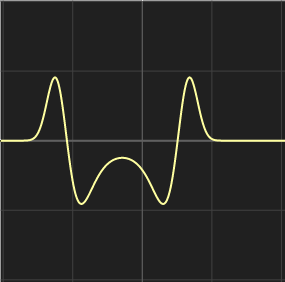
\includegraphics[width=0.25\textwidth]{images/g}
    \caption{Wykres przedstawiający funkcję opisującą zachowanie efektu Fresnela w animacji markera}
\end{figure}



\begin{lstlisting}[caption=Fragment shadera odpowiedzialny za animację]
fixed4 frag (v2f i) : SV_Target
{
  float t =  6.2 * _Progress - 0.6;
  fixed4 pattern = tex2D(_PatternTex, i.uv + _Speed *t);
  float fresnelInfluence = dot(i.worldPos, i.viewDir);
  float saturatedFresnel = saturate(1 - fresnelInfluence);

  float g = w(t, 0) - w(t, -0.2) + w(t, -1) - w(t, -1.2);
  float4 color = pow(saturatedFresnel, g * _FresnelPow) * (_Color * _ColorIntensity) * pattern;
  color.a *= dot(i.worldPos, i.viewDir);
  return color;
}
\end{lstlisting}
